\documentclass[11pt]{article}
 
\usepackage[top=0.75in, bottom=1.25in, left=1in, right=1in]{geometry} 
\usepackage{amsmath,amsthm,amssymb} %this is THE math package
\usepackage{mathtools}
\usepackage{tikz}
\usepackage{graphicx}
\usepackage{fancybox}
\usepackage{hyperref}
\usepackage{varwidth}
\usepackage{mdframed}
\usepackage{mathrsfs}
\usepackage[most]{tcolorbox}
%------------------------
%Fonts I use, uncomment if you like to use them.
%The first is the general font, and the second a math font
\usepackage{mathpazo}
\usepackage{eulervm}
%------------------------
%This is so that we have standard fonts for the double-stroked symbols
%for reals, naturals etc. regardless of what font you use.
%Don't comment
\AtBeginDocument{
  \DeclareSymbolFont{AMSb}{U}{msb}{m}{n}
  \DeclareSymbolFontAlphabet{\mathbb}{AMSb}}
%------------------------
\usepackage{graphicx}
\graphicspath{ {./images/} }

%----------------------------------------------
%User-defined environments
%Commented because we're not using them in this document
%The only uncommented ones are the Problem and Solution environment

% \newenvironment{theorem}[2][Theorem]{\begin{trivlist}
% \item[\hskip \labelsep {\bfseries #1}\hskip \labelsep {\bfseries #2.}]}{\end{trivlist}}
% \newenvironment{lemma}[2][Lemma]{\begin{trivlist}
% \item[\hskip \labelsep {\bfseries #1}\hskip \labelsep {\bfseries #2.}]}{\end{trivlist}}
% \newenvironment{exercise}[2][Exercise]{\begin{trivlist}
% \item[\hskip \labelsep {\bfseries #1}\hskip \labelsep {\bfseries #2.}]}{\end{trivlist}}
% \newenvironment{question}[2][Question]{\begin{trivlist}
% \item[\hskip \labelsep {\bfseries #1}\hskip \labelsep {\bfseries #2.}]}{\end{trivlist}}
% \newenvironment{corollary}[2][Corollary]{\begin{trivlist}
% \item[\hskip \labelsep {\bfseries #1}\hskip \labelsep {\bfseries #2.}]}{\end{trivlist}}
\newenvironment{problem}[2][Problem\!]{\begin{trivlist}
\item[\hskip \labelsep {\bfseries #1}\hskip \labelsep {\bfseries #2}]}{\end{trivlist}}
%\newenvironment{sub-problem}[2][]{\begin{trivlist}
%\item[\hskip \labelsep {\bfseries #1}\hskip \labelsep {\bfseries #2}]}{\end{trivlist}}
\newenvironment{solution}{\begin{proof}[\textbf{\textit{Solution}}] }{\end{proof}}
%----------------------------------------------

%----------------------------
%User-defined notations
\newcommand{\zz}{\mathbb Z}   %blackboard bold Z
\newcommand{\qq}{\mathbb Q}   %blackboard bold Q
\newcommand{\ff}{\mathbb F}   %blackboard bold F
\newcommand{\rr}{\mathbb R}   %blackboard bold R
\newcommand{\nn}{\mathbb N}   %blackboard bold N
\newcommand{\cc}{\mathbb C}   %blackboard bold C
\newcommand{\af}{\mathbb A}   %blackboard bold A
\newcommand{\pp}{\mathbb P}   %blackboard bold P
\newcommand{\id}{\operatorname{id}} %for identity map
\newcommand{\im}{\operatorname{im}} %for image of a function
\newcommand{\dom}{\operatorname{dom}} %for domain of a function
\newcommand{\cat}[1]{\mathscr{#1}}   %calligraphic category
\newcommand{\abs}[1]{\left\lvert#1\right\rvert} %for absolute value
\newcommand{\norm}[1]{\left\lVert#1\right\rVert} %for norm
\newcommand{\modar}[1]{\text{ mod }{#1}} %for modular arithmetic
\newcommand{\set}[1]{\left\{#1\right\}} %for set
\newcommand{\setp}[2]{\left\{#1\ \middle|\ #2\right\}} %for set with a property
\newcommand{\card}[1]{\#\,{#1}} %for cardinality of a set
\newcommand\m[1]{\begin{pmatrix}#1\end{pmatrix}} 

%Re-defined notations
\renewcommand{\epsilon}{\varepsilon}
\renewcommand{\phi}{\varphi}
\renewcommand{\emptyset}{\varnothing}
\renewcommand{\geq}{\geqslant}
\renewcommand{\leq}{\leqslant}
\renewcommand{\Re}{\operatorname{Re}}
\renewcommand{\Im}{\operatorname{Im}}
%----------------------------

\allowdisplaybreaks
 
 
\begin{document}
 
\title{11/22 Resubmission}
\author{Kevin Guillen\\[0.5em]
MATH 101 | Problem Solving | Fall 2021}
\date{} 

\maketitle
%Use \[...\] instead of $$...$$


\begin{tcolorbox}
    \begin{problem} {IC | 11/15 | 151.}
        Is it possible for a triangle to have altitudes equal to 6, 10, and 20?
    \end{problem}
\end{tcolorbox}
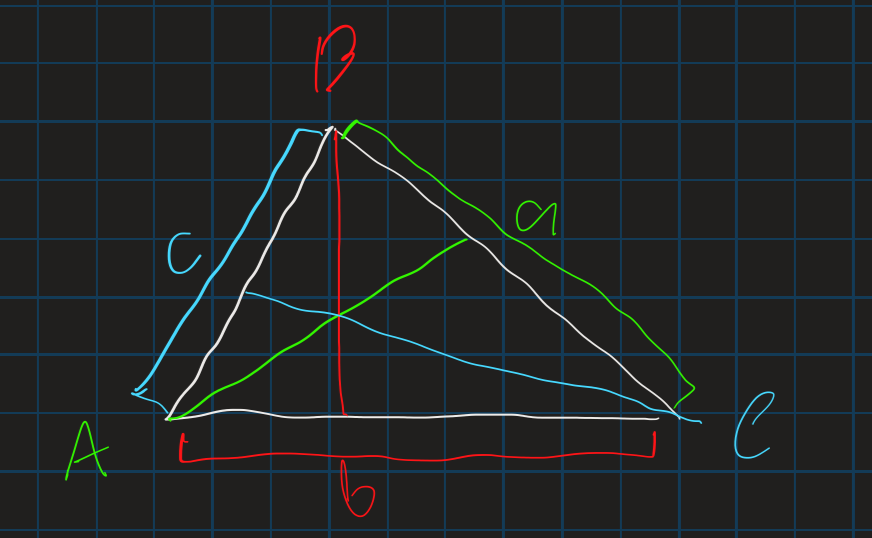
\includegraphics[scale=.5]{prob2}
\begin{proof}
    Consider the area of the triangle drawn above. It will be the following,
    \[A = \frac{6}{2}a = \frac{10}{2}b = \frac{20}{2}c.\]

    Which gives us the following equations,
    \begin{align*}
        a &= \frac{1}{3}A \\
        b &= \frac{1}{5}A \\
        c &= \frac{1}{10}A
    \end{align*}

    Recall though by the triangle inequality we have that $a < b + c$, we see through the following though,
    \begin{align*}
        a &< b + c \\
        \frac{10}{30}A &< \frac{6}{30}A + \frac{3}{10}A = \frac{9}{10}A
    \end{align*}
    that if our altitudes were 6, 10 and 20, that would imply $\dfrac{10}{30}A < \dfrac{9}{10}A$ which is a contradiction. Therefore there can not be a triangle with those given altitudes. 
\end{proof}

\begin{tcolorbox}
    \begin{problem} {OC | 11/01 | 68}
        Imagine an $n \times n$ chessboard. How many ways is it possible to choose four squares, no three in the same row or columns which are the vertices of a rectangle?
    \end{problem}
\end{tcolorbox}
\begin{proof}
    If we have an $n\times n$ chessboard that means we have $n$ columns and $n$ rows. We can treat each row and column as sides of a rectangles. If we choose 2 unique vertical lines and 2 unique horizontal lines their intersections will generate a rectangle. There are n choose 2 ways to pick our horizontal lines, and n choose 2 ways to pick our vertical lines This means for an $n \times n$ chessboard we have, 
    \[\binom{n}{2}\binom{n}{2}\]
    rectangles

\end{proof}





\begin{tcolorbox}
    \begin{problem} {OC | 11/10 | 86.}
        Prove that there are no positive integers $x$, $y$ such that $x+y$, $2x + y$, and $x + 2y$ are squares. 
    \end{problem}
\end{tcolorbox}
\begin{proof}
    Assuming this were to be true, then for integers $a$, $b$, and $c$ we have,
    \begin{align*}
        x+y &= a^{2} \\
        2x+y &= b^{2} \\
        x + 2y &= c^{2}
    \end{align*}
    Using the 2nd equation to solve for $y$ we get, $y = b^{2} -2x$. Plugging this into the 1st equation we get, $x = b^{2} - a^{2}$. Using the 1st equation to solve for $x$ we get, $x = a^{2} -y$. Pluggin this into the 2nd equation we get $y = 2a^{2} -b^{2}$.

    Now plugging in these value into the 3rd equation, we get,
    \begin{align*}
        a^{2}-y + 4a^{2} -2b^{2} &= c^{2} \\
        3a^{2} &= b^{2} + c^{2}
    \end{align*}

    Thus there is only integer solutions if this diophantine equation holds. We know any integers squared mod 4 will have values 0 or 1. Therfore $b^{2} + c^{2} \in \set{0,1,2}$, and $3a^{2}\in \set{0,3}$. This together means we must have $3a^{2} \equiv 0 \text{ mod } 4$ and $(b^{2} + c^{2}) \equiv 0 \text{ mod }4$. Meaning $a$ is even and is of the form $a = 2k$, also means that $b$ and $c$ are even and of the form $b = 2l$ and $c = 2n$. Plugging this back into the equation we get,
    \begin{align*}
        12k^{2} & = 4l^{2} + 4n^{2}.
    \end{align*}

    This means there has to be a solution for $k$, $l$, and $n$. But this can be since $k + l + n < a + b + c$. Therefore there is no integers $x$ and $y$ such that $x +y$, $2x +y$, and $x + 2y$ are squares.
\end{proof}


\end{document}